%%%%%%%%%%%%%%%%%%%%%%%%%%%%%%%%%%%%
% Slide options
%%%%%%%%%%%%%%%%%%%%%%%%%%%%%%%%%%%%

% Option 1: Slides with solutions

\documentclass[slidestop,compress,mathserif]{beamer}
\newcommand{\soln}[1]{\textit{#1}}
\newcommand{\solnGr}[1]{#1}

% Option 2: Handouts without solutions

%\documentclass[11pt,containsverbatim,handout]{beamer}
%\usepackage{pgfpages}
%\pgfpagesuselayout{4 on 1}[letterpaper,landscape,border shrink=5mm]
%\newcommand{\soln}[1]{ }
%\newcommand{\solnGr}{ }


%%%%%%%%%%%%%%%%%%%%%%%%%%%%%%%%%%%%
% Style
%%%%%%%%%%%%%%%%%%%%%%%%%%%%%%%%%%%%

\def\chp3@path{../../Chp 3}
\input{../../lec_style.tex}


%%%%%%%%%%%%%%%%%%%%%%%%%%%%%%%%%%%%
% Preamble
%%%%%%%%%%%%%%%%%%%%%%%%%%%%%%%%%%%%

\title[Lecture 7]{MA213: Lecture 7}
\subtitle{Module 2: Probability, Random Variables, and Distributions}
\author{OpenIntro Statistics, 4th Edition}
\institute{$\:$ \\ {\footnotesize Based on slides developed by Mine \c{C}etinkaya-Rundel of OpenIntro. \\
The slides may be copied, edited, and/or shared via the \webLink{http://creativecommons.org/licenses/by-sa/3.0/us/}{CC BY-SA license.} \\
Some images may be included under fair use guidelines (educational purposes).}}
\date{}

%%%%%%%%%%%%%%%%%%%%%%%%%%%%%%%%%%%%
% Begin document
%%%%%%%%%%%%%%%%%%%%%%%%%%%%%%%%%%%%

\begin{document}


%%%%%%%%%%%%%%%%%%%%%%%%%%%%%%%%%%%%
% Title page
%%%%%%%%%%%%%%%%%%%%%%%%%%%%%%%%%%%%

{
\addtocounter{framenumber}{-1} 
{\removepagenumbers 
\usebackgroundtemplate{\includegraphics[width=\paperwidth]{../../OpenIntro_Grid_4_3-01.jpg}}
\begin{frame}

\hfill \includegraphics[width=20mm]{../../oiLogo_highres}

\titlepage

\end{frame}
}
}


%%%%%%%%%%%%%%%%%%%%%%%%%%%%%%%%%%%%
% Recap/Agenda 
%%%%%%%%%%%%%%%%%%%%%%%%%%%%%%%%%%%%
% TODO better formatting
\begin{frame}
    \frametitle{Module 2: Probability, Random Variables, and Distributions}
    \begin{itemize}
        \item \hl{Previously: } Probability (Chapter 3.1)
        \item \hl{This time: } Conditional Probability, Sampling (Chapters 3.2-3.3)
        \item \hl{Reading: } Chapter 3.4 for next time
        \item \hl{Deadlines/Announcements: } 
    \end{itemize}
    
\end{frame}
    
%%%%%%%%%%%%%%%%%%%%%%%%%%%%%%%%%%%%
% Sections
%%%%%%%%%%%%%%%%%%%%%%%%%%%%%%%%%%%%

%%%%%%%%%%%%%%%%%%%%%%%%%%%%%%%%%%%%

\section{Conditional probability}

%%%%%%%%%%%%%%%%%%%%%%%%%%%%%%%%%%%%

\subsection{Exploring probabilities with a contingency table}

%%%%%%%%%%%%%%%%%%%%%%%%%%%%%%%%%%%%

\begin{frame}
\frametitle{Relapse}

Researchers randomly assigned 72 chronic users of cocaine into three groups: desipramine (antidepressant), lithium (standard treatment for cocaine) and placebo. Results of the study are summarized below.

{\small
\begin{center}
\begin{tabular}{l | c c | c}
			& 		& no 		&  \\
			& relapse	& relapse	& total \\
\hline
desipramine	& 10		& 14		& 24 \\
lithium		& 18		& 6		& 24 \\
placebo		& 20		& 4		& 24 \\
\hline
total			& 48		& 24		& 72
\end{tabular}
\end{center}
}

\ct{\webURL{http://www.oswego.edu/~srp/stats/2_way_tbl_1.htm}}

\end{frame}

%%%%%%%%%%%%%%%%%%%%%%%%%%%%%%%%%%%%

\begin{frame}

\dq{What is the probability that a patient did not relapse?}


{\small
\begin{center}
\begin{tabular}{l | c c | c}
			& 		& no 		&  \\
			& relapse	& relapse	& total \\
\hline
desipramine	& 10		& 14		& 24 \\
lithium		& 18		& 6		& 24 \\
placebo		& 20		& 4		& 24 \\
\hline
total			& 48		& 24		& 72
\end{tabular}
\end{center}
}

\end{frame}

%%%%%%%%%%%%%%%%%%%%%%%%%%%%%%%%%%%%

\subsection{Marginal and joint probabilities}

%%%%%%%%%%%%%%%%%%%%%%%%%%%%%%%%%%%%

\begin{frame}
\frametitle{Marginal probability}

\dq{What is the probability that a patient relapsed?}

{\small
\begin{center}
\begin{tabular}{l | c c | c}
			& 		& no 		&  \\
			& relapse	& relapse	& total \\
\hline
desipramine	& 10		& 14		& 24 \\
lithium		& 18		& 6		& 24 \\
placebo		& 20		& 4		& 24 \\
\hline
total			& \only<1>{48}\only<2->{\red{48}}		& 24		&  \only<1>{72}\only<2->{\red{72}}
\end{tabular}
\end{center}
}

\onslide<2->{P(relapsed) = $\frac{48}{72} \approx 0.67$} \\

\end{frame}

%%%%%%%%%%%%%%%%%%%%%%%%%%%%%%%%%%%%

\begin{frame}
\frametitle{Joint probability}

\dq{What is the probability that a patient received the antidepressant (desipramine) \underline{and} relapsed?}

{\small
\begin{center}
\begin{tabular}{l | c c | c}
			& 		& no 		&  \\
			& relapse	& relapse	& total \\
\hline
desipramine	& \only<1>{10} \only<2->{\red{10}}		& 14		& 24 \\
lithium		& 18		& 6		& 24 \\
placebo		& 20		& 4		& 24 \\
\hline
total			& 48	& 24		&  \only<1>{72} \only<2->{\red{72}}
\end{tabular}
\end{center}
}

\onslide<2->{P(relapsed and desipramine) = $\frac{10}{72} \approx 0.14$} \\

\end{frame}

%%%%%%%%%%%%%%%%%%%%%%%%%%%%%%%%%%%%

\subsection{Defining conditional probability}

%%%%%%%%%%%%%%%%%%%%%%%%%%%%%%%%%%%%

\begin{frame}
\frametitle{Conditional probability}

\formula{Conditional probability}{
The conditional probability of the outcome of interest $A$ given condition $B$ is calculated as
\[ P(A|B) = \frac{P(A~and~B)}{P(B)} \]
}

\pause

\twocol{0.5}{0.5}
{
{\small
\begin{center}
\begin{tabular}{l | c c | c}
			& 		& no 		&  \\
			& relapse	& relapse	& total \\
\hline
desipramine	& 10		& 14		& 24 \\
lithium		& 18		& 6		& 24 \\
placebo		& 20		& 4		& 24  \\
\hline
total			& 48		& 24		&  72
\end{tabular}
\end{center}
}
}
{
\begin{eqnarray*}
&&P(relapse |  desipramine) \\
&&= \frac{P(relapse ~ and ~ desipramine)}{P(desipramine)} \\
\pause
&&= \frac{10 / 72}{24 / 72} \\
\pause
&&= \frac{10}{24} \\
\pause
&&= 0.42
\end{eqnarray*}
}

\end{frame}

%%%%%%%%%%%%%%%%%%%%%%%%%%%%%%%%%%%%

\begin{frame}
\frametitle{Conditional probability (cont.)}

\dq{If we know that a patient received the antidepressant (desipramine), what is the probability that they relapsed?}

{\small
\begin{center}
\begin{tabular}{l | c c | c}
			& 		& no 		&  \\
			& relapse	& relapse	& total \\
\hline
\rowcolor[gray]{.7}
desipramine	& \only<1>{10} \only<2->{\red{10}}			& 14		& \only<1>{24} \only<2->{\red{24}} \\
lithium		& 18		& 6		& 24 \\
placebo		& 20 		& 4		& 24  \\
\hline
total			& 48	& 24		&  72
\end{tabular}
\end{center}
}

\onslide<2->{P(relapse $|$  desipramine) = $\frac{10}{24} \approx 0.42$} \\

\onslide<3->{
$\:$ \\
P(relapse $|$  lithium) = $\frac{18}{24} \approx 0.75$ \\
P(relapse $|$  placebo) = $\frac{20}{24} \approx 0.83$ \\
}

\end{frame}

%%%%%%%%%%%%%%%%%%%%%%%%%%%%%%%%%%%%

\begin{frame}
\frametitle{Conditional probability (cont.)}

\dq{If we know that a patient relapsed, what is the probability that they received the antidepressant (desipramine)?}

{\small
\begin{center}
\begin{tabular}{l | >{\columncolor[gray]{0.7}[0pt]}c c | c}
			& 		& no 		&  \\
			& relapse	& relapse	& total \\
\hline
desipramine	& \only<1>{10} \only<2->{\red{10}}			& 14		& 24 \\
lithium		& 18		& 6		& 24 \\
placebo		& 20		& 4		& 24  \\
\hline
total			& \only<1>{48} \only<2->{\red{48}}	& 24		&  72
\end{tabular}
\end{center}
}

\onslide<2->{P(desipramine $|$  relapse) = $\frac{10}{48} \approx 0.21$} \\

\onslide<3->{
$\:$ \\
P(lithium $|$  relapse) = $\frac{18}{48} \approx 0.375$ \\
P(placebo $|$  relapse) = $\frac{20}{48} \approx 0.42$ \\
}

\end{frame}

%%%%%%%%%%%%%%%%%%%%%%%%%%%%%%%%%%%
\section{Edfinity Quiz}
%%%%%%%%%%%%%%%%%%%%%%%%%%%%%%%%%%%


%%%%%%%%%%%%%%%%%%%%%%%%%%%%%%%%%%%%

\subsection{General multiplication rule}

%%%%%%%%%%%%%%%%%%%%%%%%%%%%%%%%%%%%

\begin{frame}
\frametitle{General multiplication rule}

\begin{itemize}

\item Earlier we saw that if two events are independent, their joint probability is simply the product of their probabilities. If the events are not believed to be independent, the joint probability is calculated slightly differently.

\pause

\item If $A$ and $B$ represent two outcomes or events, then
\formula{\[ P(A~and~B) = P(A|B) \times P(B) \]}
Note that this formula is simply the conditional probability formula, rearranged.
\pause

\item It is useful to think of $A$ as the outcome of interest and $B$ as the condition.

\end{itemize}

\end{frame}

%%%%%%%%%%%%%%%%%%%%%%%%%%%%%%%%%%%%

\subsection{Independence considerations in conditional probability}

%%%%%%%%%%%%%%%%%%%%%%%%%%%%%%%%%%%%

\begin{frame}
\frametitle{Independence and conditional probabilities}

Consider the following (hypothetical) distribution of gender and major of students in an introductory statistics class:

{\small
\begin{center}
\begin{tabular}{l | c c | c}
			& social	& non-social 		&  \\
			& science	& science	& total \\
\hline
female		& 30		& 20		& 50 \\
male			& 30		& 20		& 50 \\
\hline
total			& 60		& 40		& 100
\end{tabular}
\end{center}
}

\pause

\begin{itemize}

\item The probability that a randomly selected student is a social science major is \pause $\frac{60}{100} = 0.6$. 

\pause

\item The probability that a randomly selected student is a social science major given that they are female is \pause $\frac{30}{50} = 0.6$. 

\pause

\item Since $P(SS | M)$ also equals 0.6, major of students in this class does not depend on their gender: P(SS $|$ F) = P(SS).

\end{itemize}

\end{frame}

%%%%%%%%%%%%%%%%%%%%%%%%%%%%%%%%%%%%

\begin{frame}
\frametitle{Independence and conditional probabilities (cont.)}

Generically, if $P(A|B) = P(A)$ then the events $A$ and $B$ are said to be independent.

\pause

\begin{itemize}

\item Conceptually: Giving $B$ doesn't tell us anything about $A$.

\pause

\item Mathematically: We know that if events $A$ and $B$ are independent, $P(A~and~B) = P(A) \times P(B)$. Then,
\[ P(A|B) = \frac{P(A~and~B)}{P(B)} = \frac{P(A) \times P(B)}{P(B)} = P(A) \]

\end{itemize}

\end{frame}

%%%%%%%%%%%%%%%%%%%%%%%%%%%%%%%%%%%%

\subsection{Tree diagrams}

%%%%%%%%%%%%%%%%%%%%%%%%%%%%%%%%%%%%

\begin{frame}
\frametitle{Breast cancer screening}

\begin{itemize}

\item American Cancer Society estimates that about 1.7\% of women have breast cancer. \\
{\small\webURL{http://www.cancer.org/cancer/cancerbasics/cancer-prevalence}}

\item Susan G. Komen For The Cure Foundation states that mammography correctly identifies about 78\% of women who truly have breast cancer. \\
{\small\webURL{http://ww5.komen.org/BreastCancer/AccuracyofMammograms.html}}

\item An article published in 2003 suggests that up to 10\% of all mammograms result in false positives for patients who do not have cancer. \\{\small \webURL{http://www.ncbi.nlm.nih.gov/pmc/articles/PMC1360940}}

\end{itemize}

\vfill

\Note{These percentages are approximate, and very difficult to estimate.}

\end{frame}

%%%%%%%%%%%%%%%%%%%%%%%%%%%%%%%%%%%

\begin{frame}
\frametitle{Inverting probabilities}

\dq{When a patient goes through breast cancer screening there are two competing claims: patient had cancer and patient doesn't have cancer. If a mammogram yields a positive result, what is the probability that patient actually has cancer?}

\pause

\twocol{0.7}{0.3}{
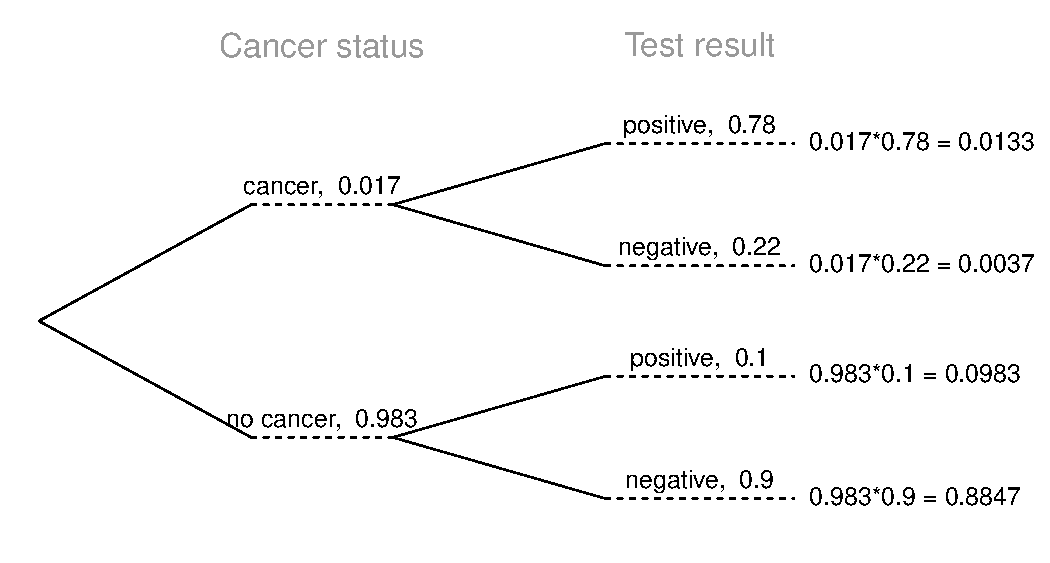
\includegraphics[width=\textwidth]{\chp3@path/3-2_conditional_probability/figures/cancer_tree/cancer_tree_first} 
}
{
\pause
{\footnotesize
\begin{eqnarray*}
&&P(C | +) \\
\pause
&&= \frac{P(C~and~+)}{P(+)} \\
\pause
&&= \frac{0.0133}{0.0133 + 0.0983} \\
\pause
&&= 0.12
\end{eqnarray*}
}
}

\pause

\Note{Tree diagrams are useful for inverting probabilities: we are given $P(+|C)$ and asked for $P(C|+)$.}

\end{frame}

%%%%%%%%%%%%%%%%%%%%%%%%%%%%%%%%%%%
\section{Edfinity Quiz}
%%%%%%%%%%%%%%%%%%%%%%%%%%%%%%%%%%%


% \begin{frame}
% \frametitle{Practice}

% \pq{Suppose a woman who gets tested once and obtains a positive result wants to get tested again. In the second test, what should we assume to be the probability of this specific woman having cancer?}

% \begin{enumerate}[(a)]
% \item 0.017
% \solnMult{0.12}
% \item 0.0133
% \item 0.88
% \end{enumerate}

% \end{frame}

%%%%%%%%%%%%%%%%%%%%%%%%%%%%%%%%%%%

% \begin{frame}
% \frametitle{Practice}

% \pq{What is the probability that this woman has cancer if this second mammogram also yielded a positive result?}

% \twocol{0.2}{0.7}
% {
% \begin{enumerate}[(a)]
% \item 0.0936
% \item 0.088
% \item 0.48
% \solnMult{0.52}
% \end{enumerate}
% }
% {
% \solnGr{\only<2->{
% 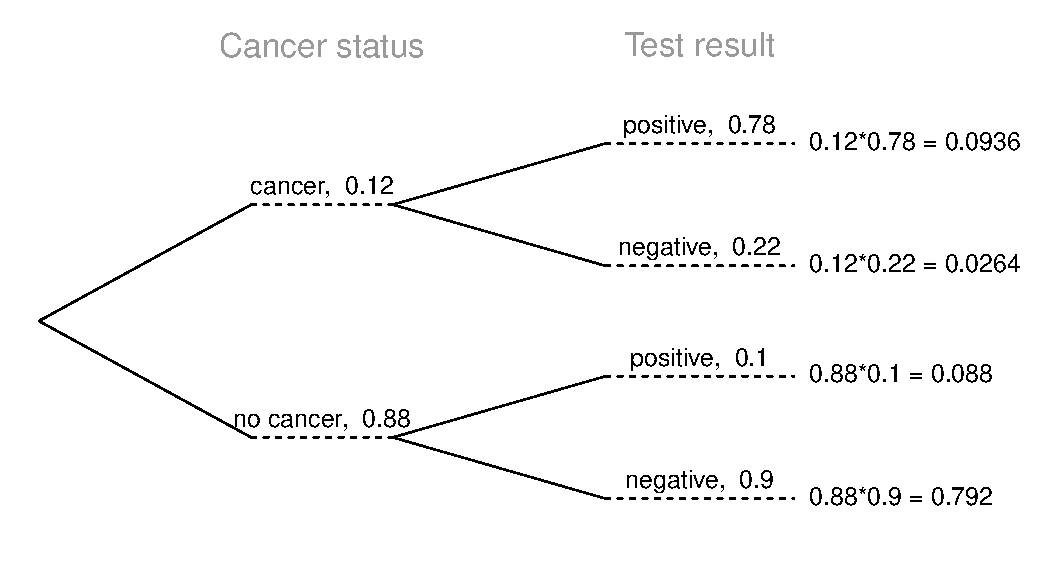
\includegraphics[width=\textwidth]{\chp3@path/3-2_conditional_probability/figures/cancer_tree/cancer_tree_second} 
% }}
% }

% \soln{\only<3->{
% {\small \[P(C | +) = \frac{P(C~and~+)}{P(+)} = \frac{0.0936}{0.0936+0.088} = 0.52\]}
% }}

% \end{frame}

%%%%%%%%%%%%%%%%%%%%%%%%%%%%%%%%%%%

\subsection{Bayes' Theorem}

%%%%%%%%%%%%%%%%%%%%%%%%%%%%%%%%%%%%

\begin{frame}
\frametitle{Bayes' Theorem}

\begin{itemize}

\item The conditional probability formula we have seen so far is a special case of the Bayes' Theorem, which is applicable even when events have more than just two outcomes.

\pause 

\item \hl{Bayes' Theorem:}
\formula{
\[ P(outcome~A_1~of~variable~1~|~outcome~B~of~variable~2) \]
\[ = \frac{P(B|A_1)P(A_1)}{P(B|A_1)P(A_1) + P(B|A_2)P(A_2) + \cdots + P(B|A_k)P(A_k)} \]
}
where $A_2$, $\cdots$, $A_k$ represent all other possible outcomes of variable 1.

\end{itemize}

\end{frame}

%%%%%%%%%%%%%%%%%%%%%%%%%%%%%%%%%%%
\section{Edfinity Quiz}
%%%%%%%%%%%%%%%%%%%%%%%%%%%%%%%%%%%

% \begin{frame}
% \frametitle{Application activity: Inverting probabilities}

% \app{{\footnotesize A common epidemiological model for the spread of diseases is the SIR model, where the population is partitioned into three groups: Susceptible, Infected, and Recovered. This is a reasonable model for diseases like chickenpox where a single infection usually provides immunity to subsequent infections. Sometimes these diseases can also be difficult to detect. \vspace{2mm} \\
% Imagine a population in the midst of an epidemic where 60\% of the population is considered susceptible, 10\% is infected, and 30\% is recovered. The only test for the disease is accurate 95\% of the time for susceptible individuals, 99\% for infected individuals, but 65\% for recovered individuals. (Note: In this case accurate means returning a negative result for susceptible and recovered individuals and a positive result for infected individuals). \vspace{2mm} \\
% Draw a probability tree to reflect the information given above. If the individual has tested positive, what is the probability that they are actually infected?
% }}

% \end{frame}

% %%%%%%%%%%%%%%%%%%%%%%%%%%%%%%%%%%%

% \begin{frame}
% \frametitle{Application activity: Inverting probabilities (cont.)}

% \vspace{-0.5cm}

% 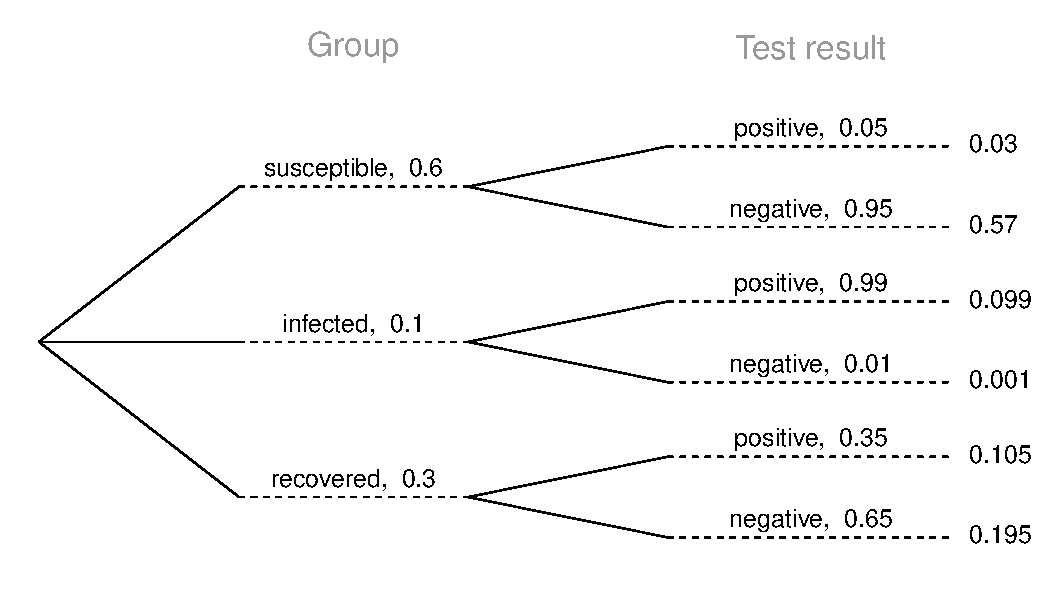
\includegraphics[width=\textwidth]{\chp3@path/3-2_conditional_probability/figures/sir_tree/sir_tree} 

% \pause

% \[ P(inf | +) = \frac{P(inf~and~+)}{P(+)} = \frac{0.099}{0.03 + 0.099 + 0.105} \approx 0.423 \]


% \end{frame}

%%%%%%%%%%%%%%%%%%%%%%%%%%%%%%%%%%%%

\section{Sampling from a small population}

%%%%%%%%%%%%%%%%%%%%%%%%%%%%%%%%%%%%

\begin{frame}
\frametitle{Sampling with replacement}

When sampling \hl{with replacement}, you put back what you just drew.

\pause

\begin{itemize}

\item Imagine you have a bag with 5 red, 3 blue and 2 orange chips in it. What is the probability that the first chip you draw is blue?
\begin{center}
5 \textcolor{red}{$\CIRCLE$}~, 3 \textcolor{blue}{$\CIRCLE$}~, 2 \textcolor{orange}{$\CIRCLE$}
\end{center}

\pause

\[ Prob(1^{st} \text{ chip } B) = \frac{3}{5 + 3 + 2} = \frac{3}{10} = 0.3 \]

\pause

\item Suppose you did indeed pull a blue chip in the first draw. If drawing with replacement, what is the probability of drawing a blue chip in the second draw?

\pause

\begin{center}
$1^{st}$ draw: 5 \textcolor{red}{$\CIRCLE$}~, 3 \textcolor{blue}{$\CIRCLE$}~, 2 \textcolor{orange}{$\CIRCLE$} \\

\pause

$2^{nd}$ draw: 5 \textcolor{red}{$\CIRCLE$}~, 3 \textcolor{blue}{$\CIRCLE$}~, 2 \textcolor{orange}{$\CIRCLE$}
\end{center}

\pause

\[ Prob(2^{nd} \text{ chip } B | 1^{st} \text{ chip } B) = \frac{3}{10} = 0.3 \]

\end{itemize}

\end{frame}

%%%%%%%%%%%%%%%%%%%%%%%%%%%%%%%%%%%%%

\begin{frame}
\frametitle{Sampling with replacement (cont.)}

\begin{itemize}

\item Suppose you actually pulled an orange chip in the first draw. If drawing with replacement, what is the probability of drawing a blue chip in the second draw?

\pause

\begin{center}
$1^{st}$ draw: 5 \textcolor{red}{$\CIRCLE$}~, 3 \textcolor{blue}{$\CIRCLE$}~, 2 \textcolor{orange}{$\CIRCLE$} \\
\pause
$2^{nd}$ draw: 5 \textcolor{red}{$\CIRCLE$}~, 3 \textcolor{blue}{$\CIRCLE$}~, 2 \textcolor{orange}{$\CIRCLE$}
\end{center}
\pause
\[ Prob(2^{nd} \text{ chip } B | 1^{st} \text{ chip } O) = \frac{3}{10} = 0.3 \]

\pause
\item If drawing with replacement, what is the probability of drawing two blue chips in a row?
\begin{center}

\pause
$1^{st}$ draw: 5 \textcolor{red}{$\CIRCLE$}~, 3 \textcolor{blue}{$\CIRCLE$}~, 2 \textcolor{orange}{$\CIRCLE$} \\
$2^{nd}$ draw: 5 \textcolor{red}{$\CIRCLE$}~, 3 \textcolor{blue}{$\CIRCLE$}~, 2 \textcolor{orange}{$\CIRCLE$}
\end{center}
\pause
\[ Prob(1^{st} \text{ chip } B) \cdot Prob(2^{nd} \text{ chip } B | 1^{st} \text{ chip } B) = 0.3 \times 0.3 \]
\[ = 0.3^2 = 0.09 \]

\end{itemize}

\end{frame}

%%%%%%%%%%%%%%%%%%%%%%%%%%%%%%%%%%%%%

\begin{frame}
\frametitle{Sampling with replacement (cont.)}

\begin{itemize}

\item When drawing with replacement, probability of the second chip being blue does not depend on the color of the first chip since whatever we draw in the first draw gets put back in the bag.
\[ Prob(B | B) = Prob(B | O) \]

\item In addition, this probability is equal to the probability of drawing a blue chip in the first draw, since the composition of the bag never changes when sampling with replacement.
\[ Prob(B | B) = Prob(B) \]

\item \hl{When drawing with replacement, draws are independent.}

\end{itemize}

\end{frame}


%%%%%%%%%%%%%%%%%%%%%%%%%%%%%%%%%%%%%

\begin{frame}
\frametitle{Sampling without replacement}

When drawing \hl{without replacement} you do not put back what you just drew.

\begin{itemize}

\pause

\item Suppose you pulled a blue chip in the first draw. If drawing without replacement, what is the probability of drawing a blue chip in the second draw?
\pause
\begin{center}
$1^{st}$ draw: 5 \textcolor{red}{$\CIRCLE$}~, 3 \textcolor{blue}{$\CIRCLE$}~, 2 \textcolor{orange}{$\CIRCLE$} \\
\pause
$2^{nd}$ draw: 5 \textcolor{red}{$\CIRCLE$}~, 2 \textcolor{blue}{$\CIRCLE$}~, 2 \textcolor{orange}{$\CIRCLE$}
\end{center}
\pause
\[ Prob(2^{nd} \text{ chip } B | 1^{st} \text{ chip } B) = \frac{2}{9} = 0.22 \]

\pause

\item If drawing without replacement, what is the probability of drawing two blue chips in a row?
\begin{center}

\pause
$1^{st}$ draw: 5 \textcolor{red}{$\CIRCLE$}~, 3 \textcolor{blue}{$\CIRCLE$}~, 2 \textcolor{orange}{$\CIRCLE$} \\
$2^{nd}$ draw: 5 \textcolor{red}{$\CIRCLE$}~, 2 \textcolor{blue}{$\CIRCLE$}~, 2 \textcolor{orange}{$\CIRCLE$}
\end{center}
\pause
\[ Prob(1^{st} \text{ chip } B) \cdot Prob(2^{nd} \text{ chip } B | 1^{st} \text{ chip } B)  = 0.3 \times 0.22 \]
\[ = 0.066 \]

\end{itemize}

\end{frame}

%%%%%%%%%%%%%%%%%%%%%%%%%%%%%%%%%%%%%

\begin{frame}
\frametitle{Sampling without replacement (cont.)}

\begin{itemize}

\item When drawing without replacement, the probability of the second chip being blue given the first was blue is not equal to the probability of drawing a blue chip in the first draw since the composition of the bag changes with the outcome of the first draw.
\[ Prob(B | B) \ne Prob(B) \]

\pause

\item \hl{When drawing without replacement, draws are not independent.}

\pause

\item This is especially important to take note of when the sample sizes are small. If we were dealing with, say, 10,000 chips in a (giant) bag, taking out one chip of any color would not have as big an impact on the probabilities in the second draw.

\end{itemize}

\end{frame}

%%%%%%%%%%%%%%%%%%%%%%%%%%%%%%%%%%%%%

% \begin{frame}
% \frametitle{Practice}

% \pq{In most card games cards are dealt without replacement. What is the probability of being dealt an ace and then a 3? Choose the closest answer.}

% \twocol{0.3}{0.6}{
% \begin{enumerate}[(a)]
% \item 0.0045
% \item 0.0059
% \solnMult{0.0060}
% \item 0.1553
% \end{enumerate}
% }
% {
% \soln{
% \pause
% \[ P(ace~then~3) = \frac{4}{52} \times \frac{4}{51} \approx 0.0060 \]
% }}

% \end{frame}

%%%%%%%%%%%%%%%%%%%%%%%%%%%%%%%%%%%%
% End document
%%%%%%%%%%%%%%%%%%%%%%%%%%%%%%%%%%%%

\end{document}